\documentclass{article}
\usepackage[T1]{fontenc}
\usepackage[utf8]{inputenc}
\usepackage{amsmath}
\usepackage{tikz}
\usepackage{tikzsymbols}
\usepackage{lmodern}
\usepackage{xcolor}
\usetikzlibrary{arrows,automata}
\setlength\parindent{0pt}

\begin{document}

\begin{center}
  \Large{Informatik D - Übungsblatt 4}

  \large{Sebastian Höffner, Andrea Suckro}
\end{center}



\section*{Aufgabe 4.1}
Automat zur Addition zweier Binärzahlen.
\begin{center}
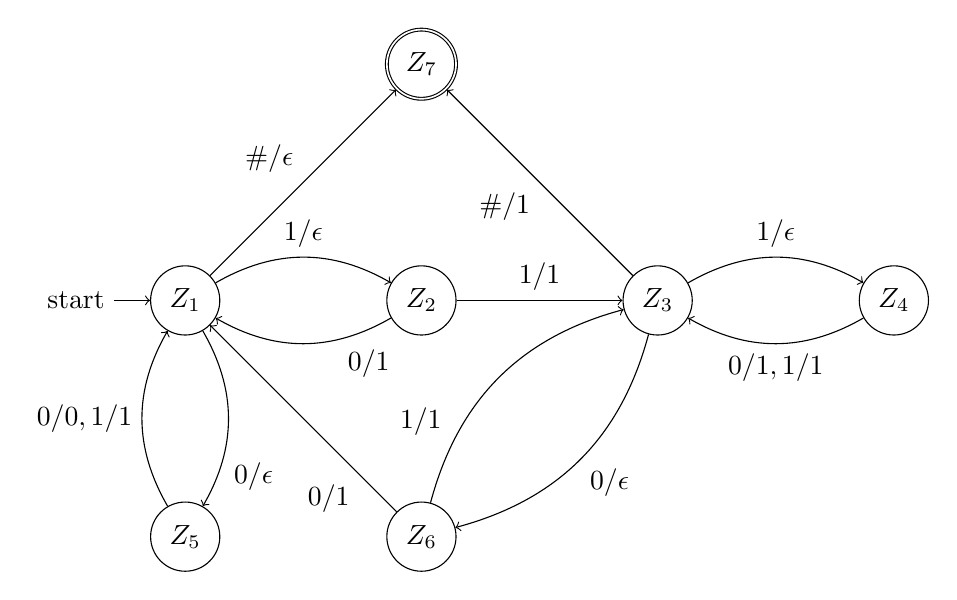
\begin{tikzpicture}[->, auto, node distance=3cm]
  \node[initial,state]   (Z1)               {$Z_1$};
  \node[state]           (Z2) [right of=Z1] {$Z_2$};
  \node[state]           (Z3) [right of=Z2] {$Z_3$};
	\node[state]           (Z4) [right of=Z3] {$Z_4$};
	\node[state]           (Z5) [below of=Z1] {$Z_5$};
	\node[state]           (Z6) [below of=Z2] {$Z_6$};
  \node[state,accepting] (Z7) [above of=Z2] {$Z_7$};

  \path (Z1) edge [bend left, pos=0.7] node {$0/\epsilon$} (Z5)
						 edge [bend left] node {$1/\epsilon$} (Z2)
             edge             node {$\#/\epsilon$}(Z7)
        (Z2) edge [bend left, pos=0.3] node {$0/1$}        (Z1)
             edge             node {$1/1$}        (Z3)
        (Z3) edge [bend left] node {$0/\epsilon$} (Z6)
             edge [bend left] node {$1/\epsilon$} (Z4)
             edge             node {$\#/1$}       (Z7)
				(Z4) edge [bend left]	node {$0/1, 1/1$}   (Z3)
				(Z5) edge [bend left]	node {$0/0, 1/1$}   (Z1)
        (Z6) edge [pos=0.2]            node {$0/1$}        (Z1)
             edge [bend left, pos=0.2] node {$1/1$}        (Z3)
        ;
\end{tikzpicture}
\end{center}


\section*{Aufgabe 4.2}

\section*{Aufgabe 4.3}

\section*{Aufgabe 4.4}

\section*{Aufgabe 4.5}

\section*{Aufgabe 4.6}




\end{document}